\section{Superconduttivit\`a}
Per introdurre la teoria della superconduttivit\`a non si pu\`o fare a meno di fare una prima panoramica sulle evidenze fenomenologiche che si sono susseguite nel corso degli anni. Le evidenze fenomenologiche hanno portato alla formulazione delle prime \textit{leggi fenomenologiche} in grado di spiegare, in modo accurato, alcune evidenze. La prima teoria fenomenologica di \textbf{London} prevedeva in modo molto buono l'espulsione di flusso di campo magnetico ma, come vedremo, aveva altri punti molto deboli. I punti deboli della teoria di London, vengono rafforzati dalla teoria fenomenologica di \textit{Ginzburg-Landau}, ammettendo quindi la possibilit\`a dell'esistenza di materiali superconduttori, in cui vi era penetrazione di campo magnetico. Su questa linea, tracciata da Ginzburg e Landau, si posiziona anche Abrikosov, con appunto l'introduzione dei famossissimi \textit{Vortici di Abrikosov}. Il tutto sfocier\`a nella realizzazione di una teria microscopica da parte di Bardeen-Cooper-Schrieffer (BCS), in cui \`e evidente che, nonostante le teorie fenomenologiche evessero dalla loro la previsione abbastanza accurata e precisa, dei fenomeni, avevano il punto di partenza completamente errato. La teoria microscopica delle coppie di Cooper apre una nuova interpretazione del fenomeno della superconduttivit\`a. 
\subsection{Evidenze Fenomenologiche}
Le evidenze fenomenologiche della superconduttivit\`a possono essere riassunte in sei punti.
\subsubsection{Evidenza della superconduttivit\`a nel Mercurio raffreddato a 4.2K}
Per semplicit\`a identifichiamo con \textbf{N} un meteriale Normale, con \textbf{S} un materiale superconduttore. Per i materiali \textbf{N}, la curva di resistivit\`a in funzione alla temperatura \`e rappresentata in modo molto buono dalla legge sperimentale
\newl{\rho(T) = \rho_o + B T^5.}
Questa dipendenza, \`e facilmente ricavabile, per esempio, facendo esperimenti di resistivit\`a sull'argento. I materiali \textbf{S} sono caratterizzati dall'esistenza di un temperatura $T_c$ chiamata \textit{temepratura critica}, tale che per $T<T_c$, la funzione di resistivit\`a scritta prima ha una discontinuit\`a e crolla a zero. Questo \`e stato il caso del Mercurio raffreddato ad una temperatura inferiore a $4.2K$. Fino a quella temperatura mostra un comportamento tipico con $\rho(T)\sim T^5$ ma da $T<T_c$, si ha che $\rho(T)=0$. Questo fatto, fu osservato per la prima volta nel 1911, dai fisici (??).

\subsubsection{Effetto Maissner-Ochsenfeld}
L'effetto Meissner-Ochsenfeld \`e un altro fatto fenomenologico, legato al fenomeno superconduttivo. Un materiale \textbf{N}, immerso in un campo magnetico, nel momento di transizione di fase per $T<T_C$ espelle quasi completamente tutto il flusso di campo magnetico che lo attraversa. Per maggior chiarezza, avviene quanto rappresentato in Fig.~\ref{MEIS:FIG}. Questo fenomeno \`e alla base della lievitazione magnetica.
\begin{figure}
	\centering
	\fbox{
	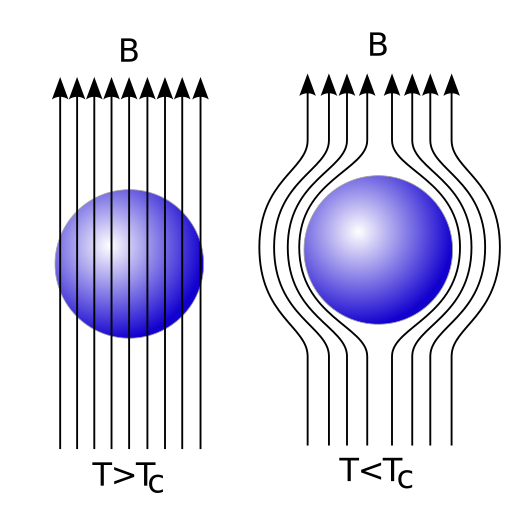
\includegraphics[width=120mm,angle=0,clip=,scale=0.5]{IMG/Meissner.png}
	}
	\caption{Rappresentazione di quello che avviene alle linee di campo magnetico per $T<T_C$}
	\label{MEIS:FIG}
\end{figure}

\subsubsection{Calore specifico}
Dal punto di vista della comprensione microscopica della superconduttivit\`a, fu particolarmente importante osservare la curva di calore specifico di un materiale superconduttore.
\begin{figure}
	\centering
	\fbox{
		\begin{tikzpicture}[scale=1,auto=center]
			\draw[->] (-2,0) -- (2,0);
			\draw[->] (-2,0) -- (-2,5);
			\node[] at (2,-0.25) {$T$};
			\node[] at (-2.5,5) {$C_v(T)$};
			\draw[domain=-2:0] plot (\x,{1.91^(\x+2)-1});
			\draw[domain=0:2] plot (\x,{0.7*\x+(2*0.7)});
			\draw[<->,dashed] (0,1.91^2-1) -- (0,-0.5); 
			\node[] at (0,-0.7) {$T_C$};
		\end{tikzpicture}
	}
	\caption{Calore specifico per un superconduttore}
	\label{SUPER:CAL:SP}
\end{figure}
Come \`e possibile osservare in Fig.~\ref{SUPER:CAL:SP}, per $T<T_C$ il calore spercifico ha un'andamento esponenziale, mentre per $T>T_C$ di tipo lineare. Questo si presta ad una interpretazione davvero affascinante in quanto \`e un diretto richiamo al modello di \textit{Cristallo di Einstein}, in pi\`u il fatto che in $T=T_C$ sia presente una discontinuit\`a, fa pensare che \textit{da qualche parte}, sia presente un gap nello spettro di energie. A chiarire questi dubbi sar\`a direttamente la teoria microscopica di BCS. La parte esponenziale per temperature inferiori alla temperatura critica, si vedr\`a essere diretta causa del fatto che la superconduttivit\`a \`e strettamente legata al verificarsi di una interazione attrattiva tra di elettroni, vicnini alla superficie di fermi, mediata da un fonone.

\subsubsection{Principio isotopico}
Il principio isotopico \`e una ulteriore prova sperimentale che il fenomeno della presenza di portatori di carica, che generano la \textit{superconrrente}, \`e strettamente legato alle interazioni col reticolo. Sperimentalmente si osserva che la temperatura critica e la massa ionica sono correlate tra loro da una legge di tipo
\newl{T_C = \frac{1}{\sqrt{M^{a^+}}}.}
Come mostrato dall'andamento del calore specifico, anche questo fatto, indica che alla base del fenomeno ci deve essere una stretta interazione col reticolo cristallino, in particolar modo, come si vedr\`a, una interazione tra gli elettroni, mediata dal fonone.

\subsubsection{Esistenza di due tipi di superconduttori}
Altra importante evidenza fenomenologica, consiste nell'esistenza di due tipi differenti di superconduttori e che il fenomeno della superconduttivit\`a \`e legato anche ad un campo mangetico critico, da cui dipende $T_C$.
Come si pu\`o notare in Fig.~\ref{SUPER:TIPI2} sono rappresentati i comportamenti dei due tipi differenti di superconduttori. Nei superconduttori di tipo II, quando si \`e tra la regione compresa tra i due campi magnetici critici, si ha uno stato misto, in cui il materiale \`e si un superconduttore ma si ha penetrazione di campo magnetico. In questa situzione di presentano i noti vortici di Abrikosov. 
\begin{figure}[H]
	\centering
	\begin{subfigure}[b]{0.4\textwidth}
	\fbox{
		\begin{tikzpicture}[scale=1,auto=center]
			\draw[->] (-2,0) -- (2,0);
			\draw[->] (-2,0) -- (-2,5);
			\node[] at (2,-0.25) {$T$};
			\node[] at (-2.75,5) {$H$};
			\draw[domain=-2:0] plot (\x,{-0.5*(\x+2)^2 +2});
			\draw[<->,dashed] (0,0.5) -- (0,-0.5); 
			\node[] at (0,-0.7) {$T_C$};
			\node[] at (-2.5,2) {$H_C$};
		\end{tikzpicture}
	}
	\caption{TIPO I - Andamento di $H_C$ in funtione a $T$. Diamagnete perfetto, completo effetto Maissner}
	\end{subfigure}
	\qquad\quad
	\begin{subfigure}[b]{0.4\textwidth}
	\fbox{
		\begin{tikzpicture}[scale=1,auto=center]
			\draw[->] (-2,0) -- (2,0);
			\draw[->] (-2,0) -- (-2,5);
			\node[] at (2,-0.25) {$T$};
			\node[] at (-2.75,5) {$H$};
			\draw[domain=-2:0] plot (\x,{-0.5*(\x+2)^2 +2});
			\draw[domain=-2:0] plot (\x,{-(\x+2)^2 +4});
			\draw[<->,dashed] (0,0.5) -- (0,-0.5); 
			\node[] at (0,-0.7) {$T_C$};
			\node[] at (-2.5,2) {$H_{C1}$};
			\node[] at (-2.5,4) {$H_{C2}$};
		\end{tikzpicture}
	}
	\caption{TIPO II - Andamento di $H_C$ in funtione a $T$. Creazione di uno stato misto. vortici di Abrikosov}
	\end{subfigure}
	\qquad\quad
        \begin{subfigure}[b]{0.4\textwidth}
	\fbox{
		\begin{tikzpicture}[scale=1,auto=center]
			\draw[->] (-2,0) -- (2,0);
			\draw[->] (-2,0) -- (-2,5);
			\node[] at (2,-0.25) {$H$};
			\node[] at (-2.75,5) {$-4\pi M$};
			\draw[domain=-2:0] plot (\x,{\x+2});
			\draw[<->,dashed] (0,1.91^2-1) -- (0,-0.5); 
			\node[] at (0,-0.7) {$H_C$};
		\end{tikzpicture}
	}
	\caption{TIPO I - Andamento della Magnetizzazione n funzione di $H$}
	\end{subfigure}
	\qquad\quad
        \begin{subfigure}[b]{0.4\textwidth}
	\fbox{
		\begin{tikzpicture}[scale=1,auto=center]
			\draw[->] (-2,0) -- (2,0);
			\draw[->] (-2,0) -- (-2,5);
			\node[] at (2,-0.25) {$H$};
			\node[] at (-2.75,5) {$-4\pi M$};
			\draw[domain=-2:0] plot (\x,{\x+2});
			\draw[domain=0:1] plot (\x,{2/(\x+1)});
			\draw[<->,dashed] (0,1.91^2-1) -- (0,-0.5); 
			\draw[<->,dashed] (1,1.91^2-1) -- (1,-0.5);
			\node[] at (0,-0.7) {$H_{C1}$};
			\node[] at (1,-0.7) {$H_{C2}$};
		\end{tikzpicture}
	}
	\caption{TIPO II - Andamento della Magnetizzazione n funzione di $H$}
	\end{subfigure}
	\caption{Comportamenti differenti dei due tipi di superconduttori}
	\label{SUPER:TIPI2}
\end{figure}

\subsubsection{Esistenza delle correnti persistenti - Intrappolamento di flusso di campo magnetico}
Una ulteriore prova dell'esistenza del fenomeno della superconduttivit\`a sono le \textit{correnti persistenti}. Supponiamo di prendere un anello di materiale superconduttore in equilibrio, immergiamolo in un campo magnetico, per effetto Meissner, si verr\`a a creare una corrente in modo tare che si venga a creare un campo magnetico che annulli quello interno. In questo regime, supponiamo di spegnere il campo magnetico esterno, quello che si verifica \`e che la corrente, non trovando modo di dissiparsi, continua a viaggiare nel materiale superconduttivo intrappolando tra la sua area, una cerca quantit\`a di campo magnetico. Si misura sperimentalmente che la quantit\`a di flusso concatenato, dovuto alle correnti persistenti \`e \textbf{quantizzato} e proporzionale a
\newl{\Phi=\frac{hc}{2e}.}
Questo risultato \`e particolarmente importante e sar\`a necessario per effettuare dei ragionamenti sulle teorie fenomenologiche che verranno esposte nel prossimo paragrafo.
\subsection{Teoria Fenomenologica di London}
La teoria fenomenologica di London \`e la prima proposta di spiegazione di spiegazione del fenomeno della superconduttivit\`a. Come sar\`a possibile vedere, presenta numerosi limiti e non spiega tutte le evidenze fenomenologiche ma deriva in modo molto preciso l'effetto Maissner per i superconduttori di tipo-I e il fatto che il flusso di campo magnetico intrappolato \`e quantizzato. Di notevole importanza sar\`a osservare la usa forma, molto simile a quella sperimentale, ma differente in un dettaglio sostanziale. London, inizia considerando che nel materiale superconduttore in studio, ci sia una certa porzione di elettroni che rappresentano i portatori di carica della supercorrente. Per semplicit\`a si identifichi questa densit\`a di super-elettroni con $n_s$, quindi la densit\`a di supercorrente \`e $J=-n_s e v$.  Si consideri che la super-corrente identificata da questi elettroni sia un fluido incomprimibile, quindi $\nabla J = 0$. Per descrivera la dinamica dei super-elettroni, si usi la legge di Lorentz
\newl{\frac{dv}{dt} = -\frac{e}{m}\left[E+\frac{1}{c}v\times B \right], }
che sviluppando la derivata totale di $v$ diventa:
\newl{\frac{dv}{dt}  + \nabla\left(\frac{1}{2}v^2\right) - v\times(\nabla \times v) = -\frac{e}{m}\left[E+\frac{1}{c}v\times B \right]. }
Riordinando semplicemente i termini
\newl{\frac{dv}{dt} + \nabla\left(\frac{1}{2} v^2\right) = -\frac{e}{m} E + v\times\left[ \nabla \times v -\frac{e}{mc}B  \right]   
	\label{LOR:SUP}
}
Si definisce Bulk della Superconduttivit\`a  la quantit\`a $Q= \nabla \times v -e/(mc)B$. Usando la seconda eq di Maxwell $\nabla \times E = -(1/c) (\partial_t B)$ \`e possibile scrivere
\newl{\frac{\partial Q}{\partial t} = \nabla \times (v\times Q).
	\label{EQUIL:SUP}
}
\`E possibile ora fare alcuni ragionamenti sulla quantit\`a $Q$. In assenza di campo magnetico, col materiale superconduttore in equilibrio, \`e sostanzialmente tutto fermo e la quantit\`a $Q=0$. Applicando un campo magnetico si ha che per effetto Maissner il superconduttore raggiunge un suo equilibrio, l'Eq.~(\ref{EQUIL:SUP}) ci indica che l'equilibrio raggiunto \`e totalmente trasparente al modo in cui lo si \`e raggiunto, quindi $Q$ rimane sempre nulla per ogni superconduttore all'equilibrio. In questo modo abbiamo le \textit{equazioni di London}, la prima deriva dal fatto che per ogni superconduttore si ha che $Q=0$,
\newl{\textbf{I Eq. London }\boxed{\nabla \times v - \frac{e}{mc}B=0.} \label{PRIM:EQ:L} }
La seconda equazione di London si determina semplicemente inserendo l'Eq.~(\ref{PRIM:EQ:L}) nel'Eq.~(\ref{LOR:SUP}) ottenendo
\newl{\textbf{II Eq. London }\boxed{\frac{dv}{dt} + \nabla\left(\frac{1}{2} v^2\right) = -\frac{e}{m}E}}
\subsubsection{Risultati della Teoria di London}
Dalla prima equazione di London si deriva subito un risultato molto importante sull'effetto Maissner. Prendiamo l'Eq.(\ref{PRIM:EQ:L}), scrivendola in funzione di $J$ compaiono una densit\`a di super-elettroni e una carica elettrica. Il rotore di $J$ \`e un laplaciano con un fattore $4\pi$. Detto questo, la prima equazione di London pu\`o essere riscritta come
\newl{\nabla^2 B(x) = \frac{mc}{4\pi n_s e^2 }B(x),}
La cui soluzione \`e particolarmente semplice
\newl{B(x) =B_0 e^{-\frac{x}{\lambda_L} },}
dove $\lambda_L$ \`e la lunghezza di penetrazione di London che nell'ordine di $\lambda_L\sim50nm$.

Sempre la prima equazione di London fornisce un'informazione molto importante sul momento dei super-elettroni. Sostituendo semplicemente, $\nabla \times A = B$ nella prima equazione di London, si ottiene che:
\newl{\nabla \times \left(p-\frac{e}{c}A\right)= \nabla \times P = 0, \label{ROT:MOM:NUL}}
che \`e un risultato che servir\`a tra poco.
Si consideri ora la seconda equazione di London linearizzata, quindi consideriamo di eliminare il termine in $\nabla v^2$
\newl{\frac{dv}{dt} = -\frac{e}{m} E, }
usando la seconda equazione di Maxwell e considerando la derivata rispetto alla densit\`a di corrente, anzich\`e le sole velocit\`a la scrittura si arricchisce divendando
\newl{\nabla\times\frac{dJ}{dt} = \frac{n_se^2}{mc}\frac{\partial B}{\partial t}.}
Integrando sulla superficie attraversata dal campo magnetico si ottiene
\newl{\int_{\Sigma} \left(\nabla\times\frac{dJ}{dt}\right) d\Sigma - \frac{n_se^2}{mc}\int_{\Sigma} \left(\frac{\partial B}{\partial t}\right) d\Sigma =0   
\\
\oint_{\gamma} \frac{dJ}{dt} dl - \frac{n_se^2}{mc} \int_{\Sigma} \left(\frac{\partial B}{\partial t}\right) d\Sigma =0
\\
\frac{d}{dt}\left( \int_{\Sigma} B \cdot d\Sigma -\frac{mc}{n_se^2}\oint_{\gamma} J \cdot dl \right)=0.
}
Si definisce \textit{FLUSSOIDE}, e lo si indica con la lettera $\Phi$, la quantit\`a
\newl{\Phi=\int_{\Sigma} B \cdot d\Sigma -\frac{mc}{n_se^2}\oint_{\gamma} J \cdot dl. \label{FLUSSOIDE}}
Ricordando l'Eq.~(\ref{ROT:MOM:NUL}) e usandola nell'Eq.~(\ref{FLUSSOIDE}) otteniamo uno dei risultati pi\`u importanti della teoria di London, cio\`e che il flusso di campo mangetico, in un superconduttore, \`e quantizzato. Facendo il conto si ottiene
\newl{\Phi=\int_{\Sigma} B \cdot d\Sigma -\frac{mc}{n_se^2}\oint_{\gamma} J \cdot dl = \int_\Sigma \left(\nabla\times A\right)\cdot d\Sigma - \frac{mc}{e}\oint_{\gamma} v\cdot dl = 
\\
=\oint_{\gamma} A \cdot dl - \frac{mc}{e}\oint_{\gamma} v\cdot dl = \oint_{\gamma}\left(A - \frac{mc}{e} v\right)\cdot dl =
\\
=-\frac{c}{e}\oint_{\gamma} \left(mv - \frac{e}{c} A\right) dl = -\frac{c}{e}\int_\Sigma\left( \nabla \times P\right) d\Sigma =0.
}
L'ultimo passaggio, applicando il teorema di Stokes, \`e esattamente l'equazione di Bohr-Sommerfeld per l'azione ridotta quantistica
\newl{0=-\frac{e}{c}\int_\Sigma\left( \nabla \times P\right) d\Sigma= -\frac{c}{e} \oint_{\gamma}P\cdot dl}
L'equazione di Bohr-Sommerfeld ha come autovalori multipli di $\hbar$, quindi risulter\`a che il flusso sar\`a multiplo di
\newl{\boxed{\Phi = \frac{n 2\pi \hbar c}{e} = \frac{hc}{e}.}}
\subsubsection{Conclusioni sulla teoria di London}
Come \`e stato possibile vedere, la teoria di London prevede bene l'esistenza dei superconduttori di tipo-I soggetti ad effetto Maissner. Prevede che la quantizzazione del flusso di campo magnetico intrappolato nel superconduttore, ma \`e sbagliato di un fattore due. Infatti, ricordando i risultati fenomenologici ottenuti con la misura del campo magnetico intrappolato in una anello superconduttore si ha che 
\newl{\Phi_{sperimentale} = 2\Phi_L.}
In questa relazione \`e riassunto il grande limite della teoria. Non spiega chi sono i portatori di carica. Non sono elettroni, sono un qualcosa con carica doppia dell'elettrone. Nonostante siano gi\`a in questo modo evidenti alcuni aspetti della superconduttivit\`a, il fatto che non siano previsti superconduttori di tipo-II e il fatto che non si riesca a valutare la natura dei portatori di carica, suggerisce il fatto che l'approcio classico al problema \`e sbagliato. Nel prossimo paragrafo si vedr\`a come questa teoria fenomenologica, pu\`o essere corretta, e raffinata inserendo le correzioni di Ginzburg-Landau all'energia libera. Nonostante gli sforzi, rimane concettualmente sbagliato il punto di partenza semi-classico di queste teoria.


















